% LaTeX support: latex@mdpi.com
% For support, please attach all files needed for compiling as well as the log file, and specify your operating system, LaTeX version, and LaTeX editor.

%=================================================================
\documentclass[metals,article,submit,pdftex,moreauthors]{Definitions/mdpi}
% For posting an early version of this manuscript as a preprint, you may use "preprints" as the journal and change "submit" to "accept". The document class line would be, e.g., \documentclass[preprints,article,accept,moreauthors,pdftex]{mdpi}. This is especially recommended for submission to arXiv, where line numbers should be removed before posting. For preprints.org, the editorial staff will make this change immediately prior to posting.

%--------------------
% Class Options:
%--------------------
%----------
% journal
%----------
% Choose between the following MDPI journals:
% acoustics, actuators, addictions, admsci, adolescents, aerobiology, aerospace, agriculture, agriengineering, agrochemicals, agronomy, ai, air, algorithms, allergies, alloys, analytica, analytics, anatomia, animals, antibiotics, antibodies, antioxidants, applbiosci, appliedchem, appliedmath, applmech, applmicrobiol, applnano, applsci, aquacj, architecture, arm, arthropoda, arts, asc, asi, astronomy, atmosphere, atoms, audiolres, automation, axioms, bacteria, batteries, bdcc, behavsci, beverages, biochem, bioengineering, biologics, biology, biomass, biomechanics, biomed, biomedicines, biomedinformatics, biomimetics, biomolecules, biophysica, biosensors, biotech, birds, bloods, blsf, brainsci, breath, buildings, businesses, cancers, carbon, cardiogenetics, catalysts, cells, ceramics, challenges, chemengineering, chemistry, chemosensors, chemproc, children, chips, cimb, civileng, cleantechnol, climate, clinpract, clockssleep, cmd, coasts, coatings, colloids, colorants, commodities, compounds, computation, computers, condensedmatter, conservation, constrmater, cosmetics, covid, crops, cryptography, crystals, csmf, ctn, curroncol, cyber, dairy, data, ddc, dentistry, dermato, dermatopathology, designs, devices, diabetology, diagnostics, dietetics, digital, disabilities, diseases, diversity, dna, drones, dynamics, earth, ebj, ecologies, econometrics, economies, education, ejihpe, electricity, electrochem, electronicmat, electronics, encyclopedia, endocrines, energies, eng, engproc, entomology, entropy, environments, environsciproc, epidemiologia, epigenomes, est, fermentation, fibers, fintech, fire, fishes, fluids, foods, forecasting, forensicsci, forests, foundations, fractalfract, fuels, future, futureinternet, futurepharmacol, futurephys, futuretransp, galaxies, games, gases, gastroent, gastrointestdisord, gels, genealogy, genes, geographies, geohazards, geomatics, geosciences, geotechnics, geriatrics, grasses, gucdd, hazardousmatters, healthcare, hearts, hemato, hematolrep, heritage, higheredu, highthroughput, histories, horticulturae, hospitals, humanities, humans, hydrobiology, hydrogen, hydrology, hygiene, idr, ijerph, ijfs, ijgi, ijms, ijns, ijpb, ijtm, ijtpp, ime, immuno, informatics, information, infrastructures, inorganics, insects, instruments, inventions, iot, j, jal, jcdd, jcm, jcp, jcs, jcto, jdb, jeta, jfb, jfmk, jimaging, jintelligence, jlpea, jmmp, jmp, jmse, jne, jnt, jof, joitmc, jor, journalmedia, jox, jpm, jrfm, jsan, jtaer, jvd, jzbg, kidneydial, kinasesphosphatases, knowledge, land, languages, laws, life, liquids, literature, livers, logics, logistics, lubricants, lymphatics, machines, macromol, magnetism, magnetochemistry, make, marinedrugs, materials, materproc, mathematics, mca, measurements, medicina, medicines, medsci, membranes, merits, metabolites, metals, meteorology, methane, metrology, micro, microarrays, microbiolres, micromachines, microorganisms, microplastics, minerals, mining, modelling, molbank, molecules, mps, msf, mti, muscles, nanoenergyadv, nanomanufacturing,\gdef\@continuouspages{yes}} nanomaterials, ncrna, ndt, network, neuroglia, neurolint, neurosci, nitrogen, notspecified, %%nri, nursrep, nutraceuticals, nutrients, obesities, oceans, ohbm, onco, %oncopathology, optics, oral, organics, organoids, osteology, oxygen, parasites, parasitologia, particles, pathogens, pathophysiology, pediatrrep, pharmaceuticals, pharmaceutics, pharmacoepidemiology,\gdef\@ISSN{2813-0618}\gdef\@continuous pharmacy, philosophies, photochem, photonics, phycology, physchem, physics, physiologia, plants, plasma, platforms, pollutants, polymers, polysaccharides, poultry, powders, preprints, proceedings, processes, prosthesis, proteomes, psf, psych, psychiatryint, psychoactives, publications, quantumrep, quaternary, qubs, radiation, reactions, receptors, recycling, regeneration, religions, remotesensing, reports, reprodmed, resources, rheumato, risks, robotics, ruminants, safety, sci, scipharm, sclerosis, seeds, sensors, separations, sexes, signals, sinusitis, skins, smartcities, sna, societies, socsci, software, soilsystems, solar, solids, spectroscj, sports, standards, stats, std, stresses, surfaces, surgeries, suschem, sustainability, symmetry, synbio, systems, targets, taxonomy, technologies, telecom, test, textiles, thalassrep, thermo, tomography, tourismhosp, toxics, toxins, transplantology, transportation, traumacare, traumas, tropicalmed, universe, urbansci, uro, vaccines, vehicles, venereology, vetsci, vibration, virtualworlds, viruses, vision, waste, water, wem, wevj, wind, women, world, youth, zoonoticdis
% For posting an early version of this manuscript as a preprint, you may use "preprints" as the journal. Changing "submit" to "accept" before posting will remove line numbers.

%---------
% article
%---------
% The default type of manuscript is "article", but can be replaced by:
% abstract, addendum, article, book, bookreview, briefreport, casereport, comment, commentary, communication, conferenceproceedings, correction, conferencereport, entry, expressionofconcern, extendedabstract, datadescriptor, editorial, essay, erratum, hypothesis, interestingimage, obituary, opinion, projectreport, reply, retraction, review, perspective, protocol, shortnote, studyprotocol, systematicreview, supfile, technicalnote, viewpoint, guidelines, registeredreport, tutorial
% supfile = supplementary materials

%----------
% submit
%----------
% The class option "submit" will be changed to "accept" by the Editorial Office when the paper is accepted. This will only make changes to the frontpage (e.g., the logo of the journal will get visible), the headings, and the copyright information. Also, line numbering will be removed. Journal info and pagination for accepted papers will also be assigned by the Editorial Office.

%------------------
% moreauthors
%------------------
% If there is only one author the class option oneauthor should be used. Otherwise use the class option moreauthors.

%---------
% pdftex
%---------
% The option pdftex is for use with pdfLaTeX. Remove "pdftex" for (1) compiling with LaTeX & dvi2pdf (if eps figures are used) or for (2) compiling with XeLaTeX.

%=================================================================
% MDPI internal commands - do not modify
\firstpage{1}
\makeatletter
\setcounter{page}{\@firstpage}
\makeatother
\pubvolume{1}
\issuenum{1}
\articlenumber{0}
\pubyear{2023}
\copyrightyear{2023}
%\externaleditor{Academic Editor: Firstname Lastname}
\datereceived{ }
\daterevised{ } % Comment out if no revised date
\dateaccepted{ }
\datepublished{ }
%\datecorrected{} % For corrected papers: "Corrected: XXX" date in the original paper.
%\dateretracted{} % For corrected papers: "Retracted: XXX" date in the original paper.
\hreflink{https://doi.org/} % If needed use \linebreak
%\doinum{}
%\pdfoutput=1 % Uncommented for upload to arXiv.org

%=================================================================
% Add packages and commands here. The following packages are loaded in our class file: fontenc, inputenc, calc, indentfirst, fancyhdr, graphicx, epstopdf, lastpage, ifthen, float, amsmath, amssymb, lineno, setspace, enumitem, mathpazo, booktabs, titlesec, etoolbox, tabto, xcolor, colortbl, soul, multirow, microtype, tikz, totcount, changepage, attrib, upgreek, array, tabularx, pbox, ragged2e, tocloft, marginnote, marginfix, enotez, amsthm, natbib, hyperref, cleveref, scrextend, url, geometry, newfloat, caption, draftwatermark, seqsplit
% cleveref: load \crefname definitions after \begin{document}

\usepackage{gensymb}
\usepackage{accents}
\usepackage{xspace}
\usepackage{tabularx}
\usepackage{lscape}
\usepackage{comment}
\usepackage{inputenc}

\usepackage[labelformat=simple]{subcaption}
\renewcommand\thesubfigure{\alph{subfigure}}
\DeclareCaptionLabelFormat{subcaptionlabel}{\normalfont(\textbf{#2}\normalfont)}
\captionsetup[subfigure]{labelformat=subcaptionlabel}

\DeclareRobustCommand{\w}{\mbox{\large\ensuremath{\mathsf{w}}}}
\DeclareRobustCommand{\dotp}{\boldsymbol{\cdot}}
\DeclareRobustCommand{\e}[1]{{\rm e}^{#1}}
\DeclareRobustCommand{\lay}[1]{^{(#1)}}
\DeclareRobustCommand{\mdot}[1]{\accentset{\mbox{\bfseries .}}{#1}}
\DeclareRobustCommand{\ie}{i.e.,\@\xspace}
\DeclareRobustCommand{\eal}{et al.\@\xspace}
\DeclareRobustCommand{\eg}{e.g.,\@\xspace}
\DeclareRobustCommand{\RMSE}{\text{E}_\text{RMS}}
\DeclareRobustCommand{\MARE}{\text{E}_\text{MAR}}
\DeclareRobustCommand{\R}{\text{R}}
\DeclareRobustCommand{\ps}{\text{s}^{-1}}
\DeclareRobustCommand{\mr}[2]{\multirow{#1}{*}{#2}}
\DeclareRobustCommand{\MPa}{\text{MPa}}

%=================================================================
% Please use the following mathematics environments: Theorem, Lemma, Corollary, Proposition, Characterization, Property, Problem, Example, ExamplesandDefinitions, Hypothesis, Remark, Definition, Notation, Assumption
%% For proofs, please use the proof environment (the amsthm package is loaded by the MDPI class).

%=================================================================
% Full title of the paper (Capitalized)
\Title{Artificial Neural Network based critical conditions for Dynamic Recrystallization of Medium Carbon Steel and Application}

%\Title{Artificial neural network based critical conditions for dynamic recrystallization initiation of medium carbon steel and Application : Analytical and Finite Element Modeling}%

% MDPI internal command: Title for citation in the left column
\TitleCitation{Artificial Neural Network based critical conditions for Dynamic Recrystallization of Medium Carbon Steel and Application}

% Author Orchid ID: enter ID or remove command
\newcommand{\orcidauthorA}{0000-0001-7367-5453}
\newcommand{\orcidauthorB}{0000-0002-1522-2787}
\newcommand{\orcidauthorC}{0000-0002-5360-5121}
\newcommand{\orcidauthorD}{0000-0002-0815-1984}
\newcommand{\orcidauthorE}{0009-0004-1420-7552}

% Authors, for the paper (add full first names)
\Author{Pierre Tize Mha $^{1}$\orcidD{}, Prashant Dhondapure $^{2}$\orcidE{}, Mohammad Jahazi $^{2}$\orcidB{}, Amèvi Tongne $^{1}$\orcidC{} and Olivier Pantalé $^{1,}$*\orcidA{}}

%\longauthorlist{yes}

% MDPI internal command: Authors, for metadata in PDF
\AuthorNames{Pierre Tize Mha, Prashant Dhondapure, Mohammad Jahazi, Amèvi Tongne, Olivier Pantalé}

% MDPI internal command: Authors, for citation in the left column
\AuthorCitation{Tize Mha, P.; Dhondapure, P.; Jahazi, M.; Tongne, A.; Pantalé, O.}
% If this is a Chicago style journal: Lastname, Firstname, Firstname Lastname, and Firstname Lastname.

% Affiliations / Addresses (Add [1] after \address if there is only one affiliation.)
\address{$^{1}$ \quad Laboratoire Génie de Production, INP/ENIT, Université de Toulouse, 47 Av d'Azereix, F-65016 Tarbes, France; ptizemha@enit.fr (P.T.M.); amevi.tongne@enit.fr (A.T.)\\
$^{2}$ \quad Department of Mechanical Engineering, École de Technologie Supérieure, 1100 Notre Dame St. W., Montréal, QC H3C 1K3, Canada; prashant-nagnath.dhondapure.1@ens.etsmtl.ca (P.D.); mohammad.jahazi@etsmtl.ca (M.J.)}

% Contact information of the corresponding author
\corres{Correspondence: olivier.pantale@enit.fr; Tel.: +33-562442933}

% Current address and/or shared authorship
%\firstnote{Current address: Affiliation 3.}
%\secondnote{These authors contributed equally to this work.}
% The commands \thirdnote{} till \eighthnote{} are available for further notes

%\simplesumm{} % Simple summary

%\conference{} % An extended version of a conference paper

% Abstract (Do not insert blank lines, i.e. \\)
\abstract{This study presents a novel and thorough approach to comprehending and simulating the DRX process during hot-compressing steel.
To achieve this goal, we studied the high-temperature deformation behavior of a medium-carbon steel through hot compression testing on a Gleeble-3800 thermomechanical simulator over a broad range of strains, strain rates, and temperatures.
We also employed an artificial neural network (ANN) to model thermo-visco-plastic behavior with a flow law.
The precision of quantifying DRX volume fraction is dependent on critical conditions, which are essential for both analytical model evaluation and numerical implementation in finite element software.
This study proposes a second ANN, serving as a universal approximator, to fit the data required for DRX critical condition calculations whereas the Johnson-Mehl-Avrami-Kohnogorov (JMAK) model served as an analytical tool to estimate the DRX volume fraction, which underwent validation through experimental measurements.
A numerical implementation of the JMAK model was conducted in ABAQUS software and compared against experimental data by means of microstructure analysis.
The comparison revealed a strong correlation between simulation and experiment.
The study investigated the impact of temperature, strain, and strain rate on DRX evolution.
The findings showed that DRX increases with rising temperature and strain, but decreases with increasing strain rate.}

% Keywords
\keyword{Artificial Neural Network; Constitutive Flow Law; Gleeble simulator, Dynamic Recrystallization, Finite Element Analysis}

% The fields PACS, MSC, and JEL may be left empty or commented out if not applicable
%\PACS{J0101}
%\MSC{}
%\JEL{}

%%%%%%%%%%%%%%%%%%%%%%%%%%%%%%%%%%%%%%%%%%
% Only for the journal Diversity
%\LSID{\url{http://}}

%%%%%%%%%%%%%%%%%%%%%%%%%%%%%%%%%%%%%%%%%%
% Only for the journal Applied Sciences
%\featuredapplication{Authors are encouraged to provide a concise description of the specific application or a potential application of the work.This section is not mandatory.}
%%%%%%%%%%%%%%%%%%%%%%%%%%%%%%%%%%%%%%%%%%

%%%%%%%%%%%%%%%%%%%%%%%%%%%%%%%%%%%%%%%%%%
% Only for the journal Data
%\dataset{DOI number or link to the deposited data set if the data set is published separately. If the data set shall be published as a supplement to this paper, this field will be filled by the journal editors. In this case, please submit the data set as a supplement.}
%\datasetlicense{License under which the data set is made available (CC0, CC-BY, CC-BY-SA, CC-BY-NC, etc.)}

%%%%%%%%%%%%%%%%%%%%%%%%%%%%%%%%%%%%%%%%%%
% Only for the journal Toxins
%\keycontribution{The breakthroughs or highlights of the manuscript. Authors can write one or two sentences to describe the most important part of the paper.}

%%%%%%%%%%%%%%%%%%%%%%%%%%%%%%%%%%%%%%%%%%
% Only for the journal Encyclopedia
%\encyclopediadef{For entry manuscripts only: please provide a brief overview of the entry title instead of an abstract.}

%%%%%%%%%%%%%%%%%%%%%%%%%%%%%%%%%%%%%%%%%%
% Only for the journal Advances in Respiratory Medicine
%\addhighlights{yes}
%\renewcommand{\addhighlights}{%

%\noindent This is an obligatory section in “Advances in Respiratory Medicine”, whose goal is to increase the discoverability and readability of the article via search engines and other scholars. Highlights should not be a copy of the abstract, but a simple text allowing the reader to quickly and simplified find out what the article is about and what can be cited from it. Each of these parts should be devoted up to 2~bullet points.\vspace{3pt}\\
%\textbf{What are the main findings?}
% \begin{itemize}[labelsep=2.5mm,topsep=-3pt]
% \item First bullet.
% \item Second bullet.
% \end{itemize}\vspace{3pt}
%\textbf{What is the implication of the main finding?}
% \begin{itemize}[labelsep=2.5mm,topsep=-3pt]
% \item First bullet.
% \item Second bullet.
% \end{itemize}
%}

%%%%%%%%%%%%%%%%%%%%%%%%%%%%%%%%%%%%%%%%%%
\begin{document}

%----------------------------------------------------------------------------------
\section{Introduction\label{sec:Introduction}}
%----------------------------------------------------------------------------------

Dynamic recrystallization is a process observed in specific materials, mainly metals and alloys, as they undergo the process of plastic deformation.
It is a phenomenon frequently seen in hot working operations, including hot rolling, hot forging, and hot extrusion.
When a metal or alloy undergoes significant plastic deformation at high temperatures, its existing grain structure is disrupted.
During the deformation process, new, smaller grains are formed, which is referred to as dynamic recrystallization (DRX).
DRX differs from static recrystallization (SRX) which takes place when there is no deformation applied on the material.
The amount of energy stored in the metal due to plastic deformation is the driving force behind the DRX process.
Typically, the newly formed grains are much smaller than the original grains of the undeformed material.
Their growth is accelerated by the stored energy and high temperatures.
DRX provides several benefits in the hot forming process by refining the grain size, enhancing the mechanical properties of the material, including strength and toughness \cite{Javidikia-2023, Shen-2021}.

As the occurrence of the DRX softens the material, the deformation loads during hot deformation must be adjusted from one pass to another to have more accurate prediction of DRX.
Therefore, understanding the critical conditions for dynamic recrystallization (DRX) is important for modeling industrial processes.
However, the extent of DRX is influenced by factors such as material composition, deformation temperature, strain rate, and strain.
By optimizing the parameters, engineers can attain the desired microstructures and mechanical properties in the final product.
Various experimental techniques have been proposed by researchers to establish DRX's critical conditions such as metallographic analysis \cite{Babu-2022}.
However, this technique requires extensive sampling before and after reaching the critical deformation point at which the material experiences recovery and recrystallization processes, resulting in the formation of new grains and a decrease in the average grain size.
Additionally, the cooling phase sometimes entails phase changes (depending on the material's type) from the hot working temperature, which alter the deformed structure, rendering the metallographic analysis complex.
Hence, simpler techniques such as the development of analytical models are required to determine DRX initiation.
In this regard, multiple studies have been carried out aiming to analytically identify the initiation of DRX.
For instance, Yan Peng \eal \cite{Peng-2022} determined the critical strain and critical stress for the DRX's initiation based on the method proposed by Najafizadeh and Jonas \cite{Najafizadeh-2006} to establish a DRX kinetic model for the hot-rolled condition based on the relationship between the characteristic parameters of DRX and temperature and strain rate. This approach defines the critical stress required for the initiation of DRX during deformation.
According to Gottstein \eal \cite{Gottstein-2004}, the critical strain for initiating DRX can also be predicted based on a work hardening model of dislocation density.
The onset of dynamic recrystallization (DRX) may be identified through the inflection point in the strain hardening rate $\theta(\sigma)=\frac{\partial \sigma}{\partial \varepsilon}$ where $\sigma$ is the stress and $\varepsilon$ is the strain.

The DRX phenomenon, based on the inflection point, was first studied by Ryan and McQueen \cite{Ryan-1989, Ryan-1990, Ryan-1990-2}.
They observed the appearance of an inflection point on the $\theta(\sigma)$ curve before the peak stress $\sigma_p$ and attributed the beginning of DRX and the critical conditions to this point.
Later, Poliak and Jonas \cite{Poliak-1996,Poliak-2003,Poliak-2003-2,Jonas-2003} confirmed the hypothesis of DRX describing the inflection point by demonstrating that it is associated with thermodynamic energy released during dislocation movements and the combination between the current dislocations with the previous one leads to the DRX's initiation.
Najafizadeh and Jonas \cite{Najafizadeh-2006} simplified Poliak and Jonas' thermodynamic model using an analytical technique to determine the critical conditions for initiating DRX.
Their widely-used approach relies on a third-degree polynomial to describe the curve $\theta(\sigma)$ and the second derivative to identify the critical stress $\sigma_c$ and strain $\varepsilon_c$.
Once calculated, the critical conditions serve as input data for the Johnson-Mehl-Avrami-Kolmogorov (JMAK) model \cite{Avrami-1939}.
This model is commonly used to estimate the volume fraction of dynamic recrystallization $X_{drx}$ during hot working.
Li \eal \cite{Li-2015} investigated the DRX properties of micro-alloyed plastic molding steel by using the Avrami kinetics model equation and the Estrin and Mecking mathematical model \cite{Estrin-1984,Mecking-1981} to determine the Avrami equation coefficients.

Zhang \eal \cite{Zhang-2016} investigated the DRX behaviors of a medium carbon alloy (Cr-Ni-Mo steel) using the Avrami kinetics model equation.
They qualitatively characterized the metallurgical properties based on variations in the Zener-Hollomon parameter.
Cho \eal \cite{Cho-2005} and Razali \eal \cite{Razali-2021} used a well-established model to predict the microstructure evolution of a Mn alloy, with a focus on DRX and grain growth phenomena.
Their results showed consistency with multiple compression tests.
Wan \eal \cite{Wan-2017} employed the same equation to predict the microstructure evolution of TiAl-based alloys during hot compression.
Li \eal \cite{Li-2018} validated the reliability of the Avrami kinetics model equation when testing the compression of Inconel 718 bolts.
Cui \eal \cite{Cui-2016} analyzed DRX by applying the Avrami kinetics model equation and discovered that the $\beta$-solidifying TiAl alloy usually started evolving at triple joints boundaries before affecting the lamellae.
Recently, Chen \eal \cite{Chen-2023} conducted a Finite Element Analysis of DRX, based on GCr15 (52100 steel) microstructure analysis, and found that temperature and strain rate have a significant impact on DRX initiation.

The precision of the critical DRX conditions is closely linked to the method of obtaining the curve $\theta(\sigma)$.
Using experimental raw data directly does not yield functional curves, thus smoothing the $\sigma(\varepsilon)$ curve as much as possible or approximating it with a polynomial function that can reproduce the curve and deducing the $\theta(\sigma)$ curve from it is commonly used.
The drawback of both of these methods is that they do not always ensure a satisfactory smoothing of the curve $\sigma(\varepsilon)$.
Nevertheless, the Universal Approximator, Artificial Neural Networks (ANN), has demonstrated effectiveness in various domains, such as predicting the flow behavior of materials like our previous work Tize Mha \eal \cite{TizeMha-2023} and many other works.
Then the predictions of $\sigma(\varepsilon)$ are used as inputs for the $\theta(\sigma)$ prediction.
Hence, this study offers a replacement of the two smoothing methods with an ANN approach to estimate the critical conditions for DRX.

%----------------------------------------------------------------------------------
\section{Materials and experiments\label{sec:MaterialsExperiments}}
%----------------------------------------------------------------------------------

The experimental tests used in this work are identical to those previously published by Tize Mha \eal \cite{TizeMha-2023}.
For additional information, readers can refer to the publications by our research group \cite{Pantale-2021}.
Nonetheless, we will outline the key aspects necessary to understand the suggested methodology.

%----------------------------------------------------------------------------------
\subsection{Experimental procedure and compression tests results\label{subsec:ExperimentalProcedure}}
%----------------------------------------------------------------------------------

The material used for this study is a medium-carbon steel with the chemical composition presented in Table \ref{tab:Composition}.
\begin{table}[H]
\centering
\caption{Chemical composition of medium carbon steel. Fe = balance.}
\newcolumntype{L}{>{\raggedright\arraybackslash}X}
\newcolumntype{C}{>{\centering\arraybackslash}X}
\begin{tabularx}{\textwidth}{LCCCCCCC}
\toprule
\textbf{Element} & \textbf{C} & \textbf{Mn} & \textbf{Mo} & \textbf{Si} & \textbf{Ni} & \textbf{Cr} & \textbf{Cu} \\
\toprule
\textbf{Wt~\%} & $0.30$ & $0.89$ & $0.52$ & $0.34$ & $0.68$ & $1.86$ & $0.17$ \\
\bottomrule
\end{tabularx}
\label{tab:Composition}
\end{table}

As detailed in Tize Mha \eal \cite{TizeMha-2023}, and reported in Figure \ref{fig:GleebleProcess}, hot compression tests were conducted on cylinders with an initial diameter of $\phi=10$~mm and a height of $h=15$~mm using a Gleeble-3800 thermomechanical simulator.
\begin{figure}[H]
\centering
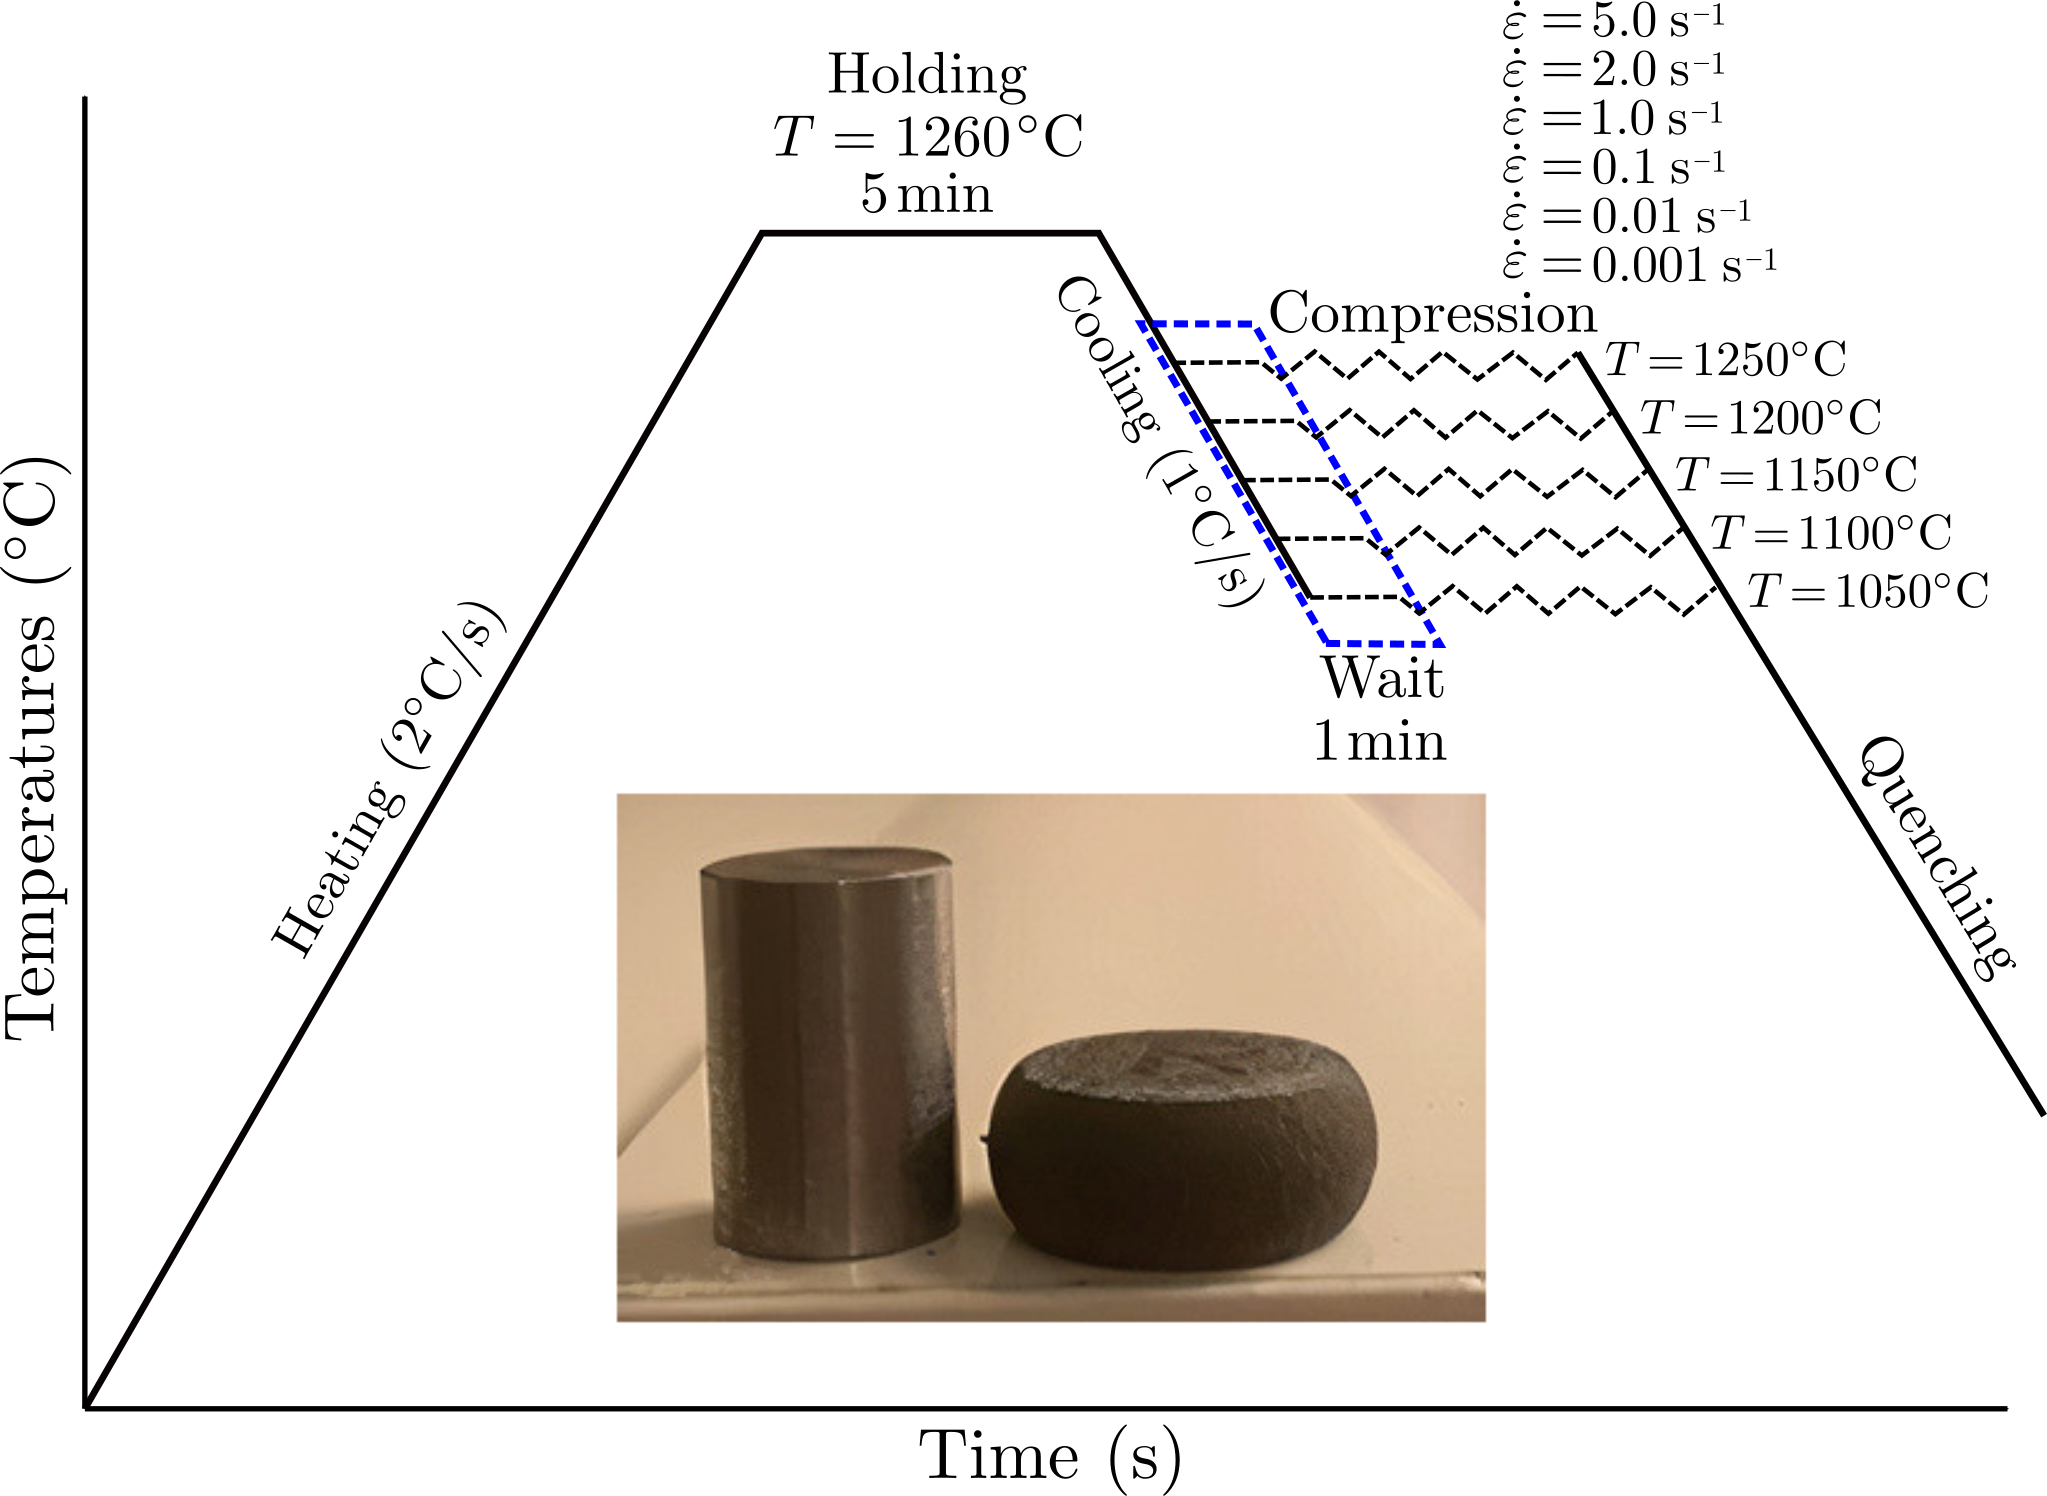
\includegraphics[width=0.7\columnwidth]{Figures/GleebleProcess}
\caption{\textls[-25]{Schematic diagram of the experimental process on the Gleeble-3800 thermomechanical simulator.}}
\label{fig:GleebleProcess}
\end{figure}
The tests were conducted at 5 temperature levels (ranging from $1050\celsius$ to $1250\celsius$) and 6 strain rates (ranging from $0.001~\ps$ to $5~\ps$).
The imposed displacement was set to $d=6$~mm, resulting in a reduction of $40\%$ of the initial height.
To reduce friction during testing, thin tantalum sheets were used as a lubricant on the contact surface of the anvils and specimens.
In order to remove thermal gradients, the samples were heated at a speed of $2$\celsius/s until reaching a temperature of $1260\celsius$, then held at that temperature for $5$~minutes.
They were subsequently cooled down to the test temperature at a speed of $1$\celsius/s and left at a consistent temperature for $1$~minute prior to being formed.
During compression, the sample temperature is maintained at a constant level through the machine's thermal control system.
Subsequently, the structure is frozen at a fast pace in order to preserve the microstructure for future analysis.

The raw stress-strain data is exported from the Gleeble thermomechanical simulator as true stress and true strain, and the set of 30 flow stress curves $\sigma$ versus strain $\varepsilon$ obtained from compression tests for each test condition is reported in Figure \ref{fig:RawData}.
All strain/stress data is composed of 701 equidistant strain values from $\varepsilon=0.0$ to $\varepsilon=0.7$ in $0.001$ increments.
\begin{figure}[H]
\centering
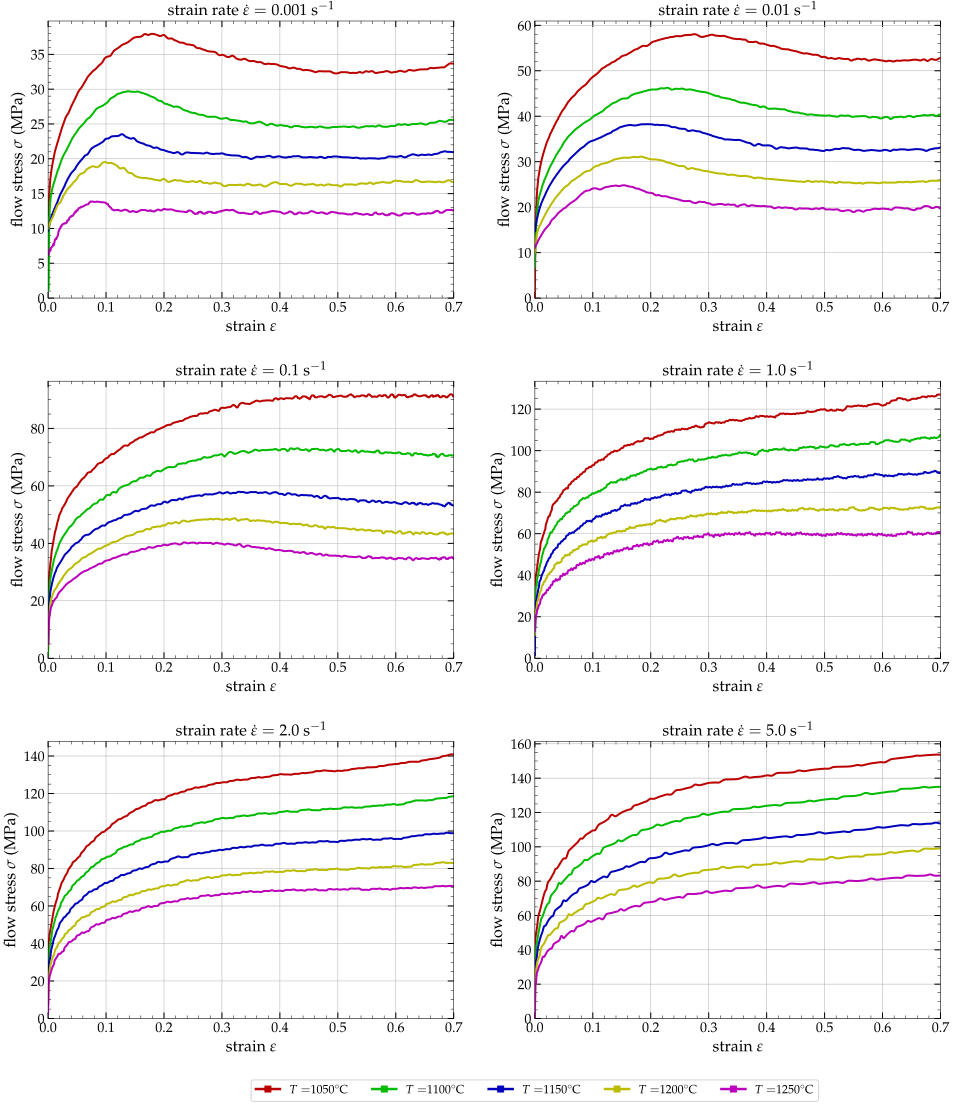
\includegraphics[width=0.9\columnwidth]{Figures/rawData}
\caption{Stress--strain curves of medium carbon alloy extracted from the Gleeble device for 5 temperatures ($T$) and 6 strain rates ($\mdot\varepsilon$).}
\label{fig:RawData}
\end{figure}

The flow stress ($\sigma$) increases as the strain rate ($\mdot\varepsilon$) rises but decreases as the temperature ($T$) increases.
Notably, the strain also affects the flow stress.
At the lowest strain rates, the flow stress increases up to $\sigma_p$ as the strain approaches a value of about $\varepsilon_p=0.2$ to $0.3$.
Then, it decreases to maintain a relatively constant value throughout the entire test.
Conversely, at strain rates above $1~\ps$, the flow stress increases steadily throughout the test.
The nominal rise in stress observed at low strain rates with large strain values is attributed to friction between the sample and anvil during testing, as noted by Galos \eal \cite{Galos-2022}.
Furthermore, this frictional effect becomes more apparent as lubrication reduces over time as reported in Tize Mha \eal \cite{TizeMha-2023}.

The initial increase in stress seen during deformation up to $\varepsilon=0.1$ is believed to be due to work hardening (WH).
After $\varepsilon=0.1$ up to $0.2$, the flow stress indicates a steady decrease as the stress level rises until a peak or inflection point is attained.
This peak suggests that thermal softening is now the predominant influence, overtaking work hardening.
At this stage, the stress-strain curve displays three distinct patterns as strain increases.
The first pattern is a gradual decrease to a steady state with DRV/DRX softening, which is observed at all deformation temperatures and strain rates ranging from $\mdot\varepsilon=0.001~\ps$ to $0.1~\ps$, except at $1050\celsius$ and $1100\celsius$.
The second pattern is higher stress levels without significant softening and work hardening at $1050\celsius$ and $1100\celsius$ with a strain rate of $0.1~\ps$.
The last pattern is a continuous increase with significant work hardening observed for all deformation temperatures and a strain rate above $1~\ps$.
This indicates that DRX softening happens at high temperatures and low strain rates,
and the rate of softening due to DRX slows down at higher strain rates and lower temperatures due to higher work hardening rates.
The result is that both the peak stress $\sigma_p$ and the onset of steady-state flow occur at higher strain levels.
The decrease in stress detected across all temperatures and strain rates of $\mdot\varepsilon=0.001-5.0~\ps$ is attributed to the event of dynamic recrystallization (DRX).

%----------------------------------------------------------------------------------
\subsection{DRX model's parameters identification\label{subsec:DRXParameters}}
%----------------------------------------------------------------------------------

In this subsection we will determine the critical deformation required to initiate recrystallization.
Ryan and McQueen \cite{Ryan-1989, Ryan-1990, Ryan-1990-2} were the pioneers in investigating this phenomenon.
Observing the appearance of an inflection point on the curve $\theta(\sigma)=\frac{\partial \sigma}{\partial \varepsilon}$ before the peak stress $\sigma_p$, the start of DRX was attributed to this inflection point, and therefore the critical values of the strain ($\varepsilon_c$) and stress ($\sigma_c$) respectively.
Later, Poliak and Jonas \cite{Poliak-1996, Poliak-2003, Poliak-2003-2, Jonas-2003} demonstrated that this inflection point is associated with a release of thermodynamic free energy during dislocation motion, supporting the DRX hypothesis.
Najafizadeh and Jonas \cite{Najafizadeh-2006} developed an analytical technique to determine the critical conditions for DRX initiation, simplifying the thermodynamic model of Poliak and Jonas.
Their widely-used approach adopts a $3^\text{rd}$ degree polynomial to describe the curve $\theta(\sigma)$, enabling the identification of critical stress and strain ($\sigma_c$ and $\varepsilon_c$) through the second derivative.

As previously stated, critical values for DRX initiation are determined by identifying the inflection point on the $\theta(\sigma)$ curve between $\varepsilon=0$ and $\varepsilon_c$.
One challenge is calculating the derivative of stress versus strain values numerically, as compression test data exhibits oscillations, as depicted in Figure \ref{fig:RawData}.
It is not feasible to compute the derivative $\theta(\sigma)=\frac{\partial \sigma}{\partial \varepsilon}$ directly.

To overcome this difficulty, certain authors propose smoothing out the empirical data (perhaps through the utilization of the Excel solver \cite{Najafizadeh-2006}) or discovering an analytical function (such as a polynomial with a relatively high degree) through a minimization algorithm.
But, depending on the degree of the polynomial and for the same stress/strain curve, multiple solutions may be obtained.
This results in multiple possible forms for the $\theta(\sigma)$ function.

%----------------------------------------------------------------------------------
\subsubsection{ANN based filtering model's architecture\label{subsec:ANNbasics}}
%----------------------------------------------------------------------------------

To improve the results obtained through the process of identifying critical values, we suggest employing the universal approximator capability of artificial neural networks.
This can be done by characterizing each strain-hardening curve using an ANN with just one input (strain) and one output (stress).
In this type of network, each layer of neurons is linked to the preceding and subsequent layers through weighted connections.
Any hidden layer $k$, containing $n$ neurons, takes a weighted sum of the outputs $\overrightarrow{\hat{y}}$ of the immediately preceding layer $(k-1)$, containing $m$ neurons, given by the following~equation:
\begin{equation}
y_i\lay{k} = \sum_{j=1}^m w_{ij}\lay{k} \hat{y}_j^{(k-1)}+ b_i\lay{k},\label{eq:ANN1}
\end{equation}
where $y_i\lay{k}$ is the entry of the $i$th neuron of layer $k$, $\hat{y}_j\lay{k-1}$ is the output of the $j$th neuron of layer $(k-1)$, $w_{ij}\lay{k}$ is the associated weight parameter between the $i$th neuron of layer $k$ and the $j$th neuron of layer $(k-1)$, and $b_i\lay{k}$ is the associated bias of the $i$th neuron of layer $k$.
Those weights $w_{ij}$ and bias $b_i$, for each layer, are the training parameters of the ANN, which we have to adjust during the training procedure.
For the proposed model, we selected the Sigmoid activation function, so that each neuron in the hidden layer $k$ provides an output value ${\hat{y}}$ from the input value $y$ of the same neuron defined by Equation (\ref{eq:ANN1}) according to the following equation:
\begin{equation}
\hat{y}=\frac{1}{1 + \e{-y}}\label{eq:ANN2}
\end{equation}

No activation function was used for the output neuron of the ANN, as is typically omitted in regression applications.
The chosen architecture for our application consists of two hidden layers, one with 7 neurons and the other with 5 neurons, as illustrated in Figure \ref{fig:ANN-7-5}.
To calculate the number of internal parameters $N_{int}$ in the model, where $n$ and $m$ represent the number of neurons in the first and second hidden layers, respectively, the following formula may be used: $N_{int}=m(2+n)+2n+1$.
So that for a $7-5$ network, $N_{int}=60$.
\begin{figure}[H]
\centering
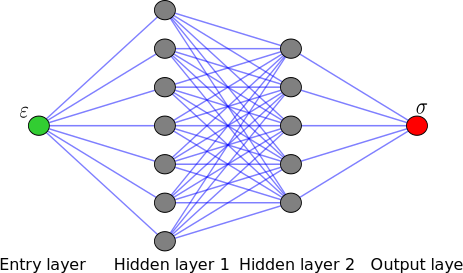
\includegraphics[width=0.7\columnwidth]{Figures/ANN-7-5}
\caption{Two hidden layers artificial neural network architecture with 1 input neuron (green) and 1 output neuron (red).}
\label{fig:ANN-7-5}
\end{figure}
The Python program used for training the neural network was created with the dedicated Python library, Tensorflow \cite{Abadi-2016}.
The training phase employed the Adaptive Moment Estimation (ADAM) optimizer \cite{Kingma-2015}.
The training was conducted using $50,000$ epochs of the experimental dataset.
It took approximately 15 minutes to train the ANN model on a Dell XPS-13 7390 laptop running Ubuntu 22.04 LTS 64-bit with 16 GB of RAM and an Intel 4-core i7-10510U processor until the converged parameters were obtained.

%----------------------------------------------------------------------------------
\subsubsection{ANN filtering based model's application \label{subsec:ANNapplication}}
%----------------------------------------------------------------------------------

Since the dynamic recrystallization phenomenon only occurs for strain rates between $0.001~\ps$ and $1.0~\ps$, we will use only the first 20 stress/strain curves to identify the DRX critical parameters.
Each of these 20 curves consists of 701 pairs of strain-stress values and was independently processed by a neural network, resulting in the identification of 20 networks.
As an example, Figure \ref{fig:AnnFit} displays the stress/strain curve experimental values for $\mdot\varepsilon=0.001~\ps$ and $T=1050\celsius$ (in blue) and the neural network results identified from this data (in red).

\begin{figure}[H]
\centering
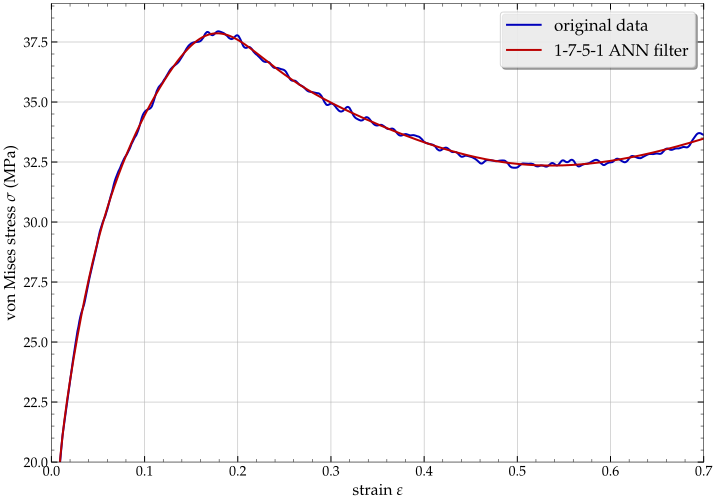
\includegraphics[width=0.7\columnwidth]{Figures/AnnFit}
\caption{Filtering of the stress/strain data using the ANN for $\mdot\varepsilon=0.001~\ps$ and $T=1050\celsius$.}
\label{fig:AnnFit}
\end{figure}
The models' accuracy and predictive ability are typically evaluated using specific coefficients, such as the mean absolute relative error ($\MARE$), as defined by the following equation:
\begin{equation}
\MARE(\%) = \frac{1}{N} \sum_{i=1}^{N}{\left|\frac{\sigma_i^p -\sigma_i^e}{\sigma_i^e}\right|} \times 100, \label{eq:AARE}
\end{equation}
and the root-mean-squared error ($\RMSE$) defined by the following equation:
\begin{equation}
\RMSE (\MPa) = \sqrt{\frac{1}{N} \sum_{i=1}^{N} \left(\sigma_i^p - \sigma_i^e\right)^2}, \label{eq:RMSE}
\end{equation}
where $\sigma_i^e$ is the experimental value, $\sigma_i^p$ is the value of the stress $\sigma$ predicted using the given model, and $N$ is the total number of data points used to compute those coefficients.
For the proposed ANN filter $\RMSE=0.093~\MPa$ and $\MARE=0.231~\%$, while using a $11^{th}$ order polynomial fit of the experimental data leads to $\RMSE=0.120~\MPa$ and $\MARE=0.275~\%$.

It is evident that using the ANN model to depict the $\sigma(\varepsilon)$ curve is superior to using an $11^{th}$ order polynomial fit, as demonstrated by the lower estimated error.
Thus, this architecture of the ANN model is used for all subsequent curves, resulting in the deduction of the hardening curves, which illustrate the stress change rate relative to strain ($\frac{\partial \sigma}{\partial \varepsilon}$).
An illustration of computing the hardening curve $\theta(\sigma)$ for a single temperature is displayed in Figure \ref{fig:AnnTheta}.
The blue line represents the direct calculation of the derivative of the raw stress versus strain, whereas the red line represents the derivative of the stress filtered by the neural network versus strain.
An overview of the remaining temperatures can be found in Figure \ref{fig:nThetaOP}.
The identical process applies to all 20 stress/strain curves.
These curves deliver essential data regarding the critical stresses and strains required for predicting DRX in the subsequent analysis.

\begin{figure}[H]
\centering
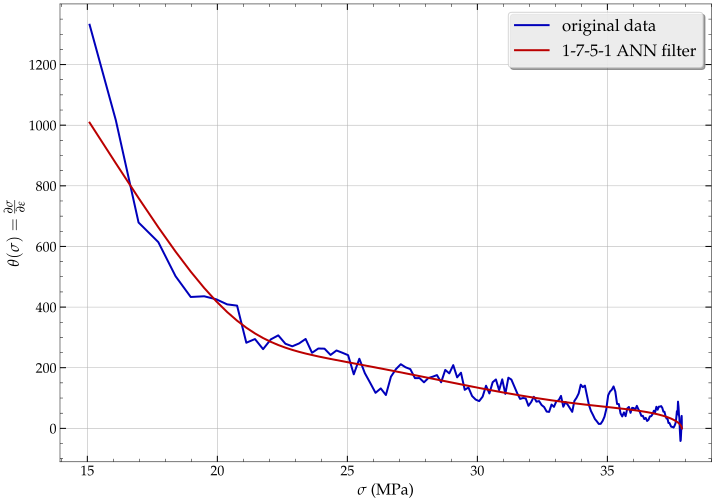
\includegraphics[width=0.7\columnwidth]{Figures/AnnTheta}
\caption{Computation of the hardening curve $\theta(\sigma)$ from the stress/strain data using the ANN for $\mdot\varepsilon=0.001~\ps$ and $T=1050\celsius$.}
\label{fig:AnnTheta}
\end{figure}

\begin{figure}[H]
\centering
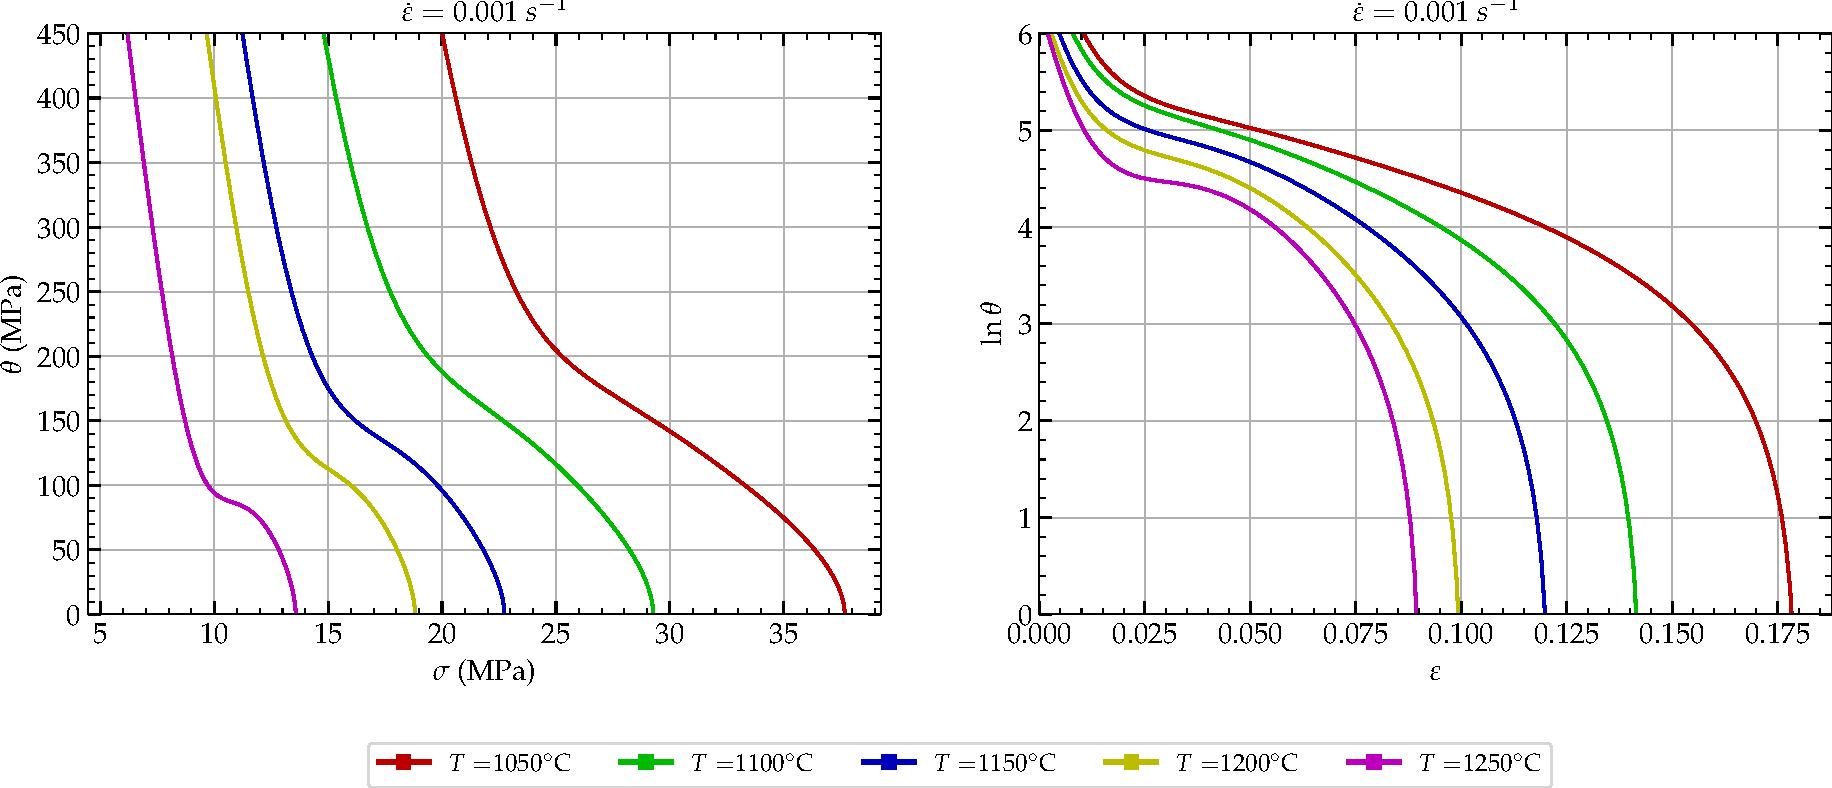
\includegraphics[width=0.99\columnwidth]{Figures/nThetaOP}
\caption{Work hardening computation for one strain rate and five temperatures.}
\label{fig:nThetaOP}
\end{figure}

%----------------------------------------------------------------------------------
\subsubsection{Critical conditions evaluation\label{subsec:CrConditions}}
%----------------------------------------------------------------------------------

As described previously, dynamic recrystallization only occurs when a particular critical condition is met.
The identification of these critical conditions is a difficult task that calls for the creation of models that can compute the corresponding critical stress and strain.
Consequently, the Poliak and Jonas \cite{Poliak-1996,Poliak-2003,Poliak-2003-2,Jonas-2003} method, which is currently well-regarded, will be used in this investigation.
The method uses a third-degree polynomial function to describe the $\theta(\sigma)$ and $\ln \theta(\varepsilon)$ curves reported in Figure \ref{fig:nThetaOP} for $\mdot\varepsilon=0.001~\ps$.
The objective is to locate the inflection points connected to the critical stress $\sigma_c$ and critical strain $\varepsilon_c$, as well as to extract the peak stress $\sigma_p$ and peak strain $\varepsilon_p$ from those curves.

The determination of critical values is carried out in two consecutive steps for each of the curves.
Firstly, based on the definition of the $\theta(\sigma)$ curve as depicted in Figure \ref{fig:nThetaOP}, we use the polyfit method from the numpy library to determine the optimal values of the constants $a_i$ for a third-degree polynomial function $p(\sigma)$ approximating $\theta(\sigma)$:
\begin{equation}
p(\sigma) = a_0\sigma^3 + a_1\sigma^2 + a_2\sigma + a_3
\end{equation}
Secondly, the inflection point $\sigma_c$ can be obtained from the second derivative of $p(\sigma)$ with:
\begin{equation}
\frac{d^2 p(\sigma)}{d \sigma^2} = 0 \Longrightarrow \sigma_c = -a_1/3a_0
\end{equation}
Similarly, the critical strain ($\varepsilon_c$) is calculated by defining a third-degree polynomial function $q(\sigma)$ approximating the $\ln \theta(\varepsilon)$ curve as depicted in Figure \ref{fig:nThetaOP}:
\begin{equation}
q(\varepsilon) = b_0\varepsilon^3 + b_1\varepsilon^2 + b_2\varepsilon + b_3
\end{equation}
This later gives the critical strain $\varepsilon_c$ from $\varepsilon_c = -b_1/3b_0$.
Applying the identical method to the first four strain rates and all temperatures, Table \ref{tab:OPparams} summarizes the critical stress and strain, peak stress, and peak strain.
Once the critical DRX conditions are established, they can be used as input to determine the DRX volume fraction, which will be discussed in the following section.

\begin{table}[h!]
\centering
\caption{Critical conditions based on the proposed approach.}\vspace{-1mm}
\begin{tabular}{cccccc}
\toprule
$\mdot{\varepsilon}$ ($\ps$) & $T$ (\celsius) & $\varepsilon_p$ & $\sigma_p$ (MPa) &  $\varepsilon_c$ & $\sigma_c$ (MPa) \\
\toprule
 & $1050$ & $0.178$ & $37.862$ & $0.083$ & $33.050$\\
 & $1100$ & $0.143$ & $29.770$ & $0.067$ & $25.648$\\
$0.001$ & $1150$ & $0.124$ & $23.330$ & $0.051$ & $19.116$\\
 & $1200$ & $0.102$ & $19.373$ & $0.039$ & $16.244$\\
 & $1250$ & $0.084$ & $13.883$ & $0.035$ & $11.302$\\
\hline
 & $1050$ & $0.281$ & $57.915$ & $0.131$ & $51.602$\\
 & $1100$ & $0.228$ & $46.107$ & $0.108$ & $40.495$\\
$0.01$ & $1150$ & $0.195$ & $38.249$ & $0.086$ & $33.435$\\
 & $1200$ & $0.172$ & $30.991$ & $0.076$ & $26.718$\\
 & $1250$ & $0.139$ & $24.739$ & $0.051$ & $20.004$\\
\hline
 & $1050$ & $0.571$ & $91.413$ & $0.244$ & $83.814$\\
 & $1100$ & $0.430$ & $72.662$ & $0.194$ & $65.259$\\
$0.1$ & $1150$ & $0.344$ & $57.774$ & $0.160$ & $51.723$\\
 & $1200$ & $0.299$ & $48.473$ & $0.136$ & $42.386$\\
 & $1250$ & $0.259$ & $40.195$ & $0.119$ & $35.277$\\
\hline
 & $1050$ & $0.700$ & $127.17$ & $0.577$ & $116.10$\\
 & $1100$ & $0.700$ & $106.61$ & $0.329$ & $94.510$\\
$1$ & $1150$ & $0.700$ & $89.525$ & $0.268$ & $89.067$\\
 & $1200$ & $0.700$ & $72.270$ & $0.178$ & $57.929$\\
 & $1250$ & $0.393$ & $59.992$ & $0.112$ & $54.066$\\
\bottomrule
\end{tabular}
\label{tab:OPparams}
\end{table}

%----------------------------------------------------------------------------------
\subsection{DRXmodel parameters evaluation\label{subsec:DRXparams}}
%----------------------------------------------------------------------------------

The DRX process commences at a critical deformation, as previously noted.
The degree of recrystallization can be determined through experimental means.
%Figure \ref{fig:DRXschema} depicts three phases of recrystallization: nucleation, grain growth, and grain coalescence \cite{Wan-2017}.
%\begin{figure}[!ht]
%\centering
%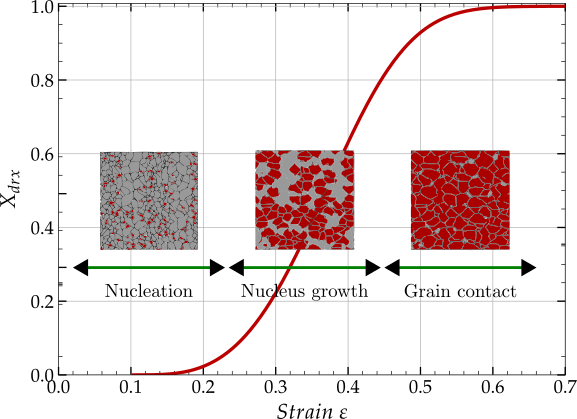
\includegraphics[width=0.7\columnwidth]{Figures/picDRX}
%\caption{Schematic diagram of three stages during DRX, nucleation, nucleus growth and grain contact.}
%\label{fig:DRXschema}
%\end{figure} 
For some visual representation of microstructure evolution during DRX, the interested reader can refer to Chen \eal \cite{Chen-2019}.

The flow stress curve of the material is influenced by the rate of work hardening, which in turn is affected by dislocations within the free grains.
The predicted volume fraction of the dynamic recrystallization ($X_{drx}^{p}$) is estimated using the Avrami model \cite{Avrami-1939} , commonly known as the JMAK model, expressed by the following equation:
\begin{equation}
X_{drx}^{p} = 1 - \exp\left[ -k\left(\frac{\varepsilon - \varepsilon_c}{\varepsilon_p}\right)^{n_k}\right]
\label{eq:drxpred}
\end{equation}
With $\varepsilon_c$ and $\varepsilon_p$ as the critical and peak strain respectively; $k$ and $n_k$ as the model's parameters and the experimental equivalence of this volume fraction of DRX is given by :
\begin{equation}
X_{drx}^{e} = \frac{\sigma_p-\sigma}{\sigma_p-\sigma_{s}}
\label{eq:drxexp}
\end{equation}

Where $\sigma_p$ and $\sigma_s$ are the peak stress and the steady stress after the peak stress respectively.
The steady stress is considered as the minimum one after the peak stress.
It is possible to establish a dependency relationship between these specific stresses/strains and the Zener-Hollomon \cite{Zenner-1944} parameter $Z = \mdot\varepsilon \exp{\left(\frac{Q}{RT}\right)} \label{eq:ArZ}$, (where $Q$ is the effective activation energy parameter $Q=437.4~\text{kJ/mol}$, $R$ is the universal gas constant $R=8.314~\text{J/mol/K}$), according to the following equation reported by other researchers such as \cite{Chen-2014,Li-2019,Wang-2021} for similar steel compositions and deformation conditions:
\begin{equation}
\begin{cases}
\varepsilon_c = A_cZ^{n_c} \\ \varepsilon_p = A_pZ^{n_p} \\ \sigma_c = B_cZ^{m_c} \\ \sigma_p = B_pZ^{m_p}\\ \sigma_s = B_sZ^{m_s},
\end{cases}
\label{eq:paramsZ}
\end{equation}
with the parameters $A_c$, $A_p$, $n_c$, $n_p$, $B_c$, $B_p$, $B_s$, $m_c$, $m_p$, and $m_s$, the specific strains and stresses' dependency on the Zener-Hollomon parameter whose identification is described here after.
The procedure for determining of the value of $Q$ is detailed in \cite{TizeMha-2023}.

The JMAK model's parameter identification involves two main steps, starting with determining the 10 coefficients $A$, $n$, $B$, and $m$.
Secondly, those coefficients are integrated into equation (\ref{eq:paramsZ}) to be used in equations (\ref{eq:drxpred}) and (\ref{eq:drxexp}).
To calculate these parameters, the curve\_fit method of the scipy library is employed through a Python code.
These parameter identifications use the critical strains and stresses computed in the preceding sections as input data.
The curve-fitting method seeks to obtain optimal values for the coefficients by iteratively adjusting them to minimize the gap between predicted and actual critical strains and stresses.
This optimization process entails experimenting with different combinations of coefficients and assessing their appropriateness for the provided data.
The curve-fitting technique fine-tunes coefficients until it attains the most accurate match between the model's forecasts and the experimental data.

Once the calculation of the constants that define the dependency of the Zener-Hollomon parameter is completed, an optimization technique can be employed to deduce the JMAK model parameters while minimizing the error between the predicted recrystallization $X_{drx}^{p}$ and the experimental value $X_{drx}^{e}$.
Table \ref{tab:allparams} displays the dependency of both the Zener-Hollomon parameters and the JMAK model parameters.

\begin{table}[h]
\centering
\caption{JMAK model and Zener-Hollomon dependency parameters.}\vspace{-1mm}
\begin{tabular}{cccccc}
\toprule
$A_c$ & $A_p$& $B_c$& $B_p$& $B_s$& $n_c$ \\
\hline
$4.4268\times10^{-5}$& $29.85\times10^{-5}$& $0.0720627$&$0.103141$&$10265.8$&$0.235832$\\
\toprule
$n_p$ & $m_c$& $m_p$& $m_s$& $k$& $n_k$ \\
\hline
$0.203678	$& $0.188236$&$0.181822$&$-0.19708$&$0.48632$&$3.36531$\\
\bottomrule
\end{tabular}
\label{tab:allparams}
\end{table}

The critical conditions calculated by the Poliak method are used to provide the curves of $X_{drx}(\varepsilon)$ in Figure \ref{fig:nDRX} where comparison between experimental and prediction is made for strain rate $\mdot\varepsilon=0.001~\ps$ and three temperature ($1050^\circ$C, $1150^\circ$C and $1250^\circ$C).
\begin{figure}[H]
	\centering
	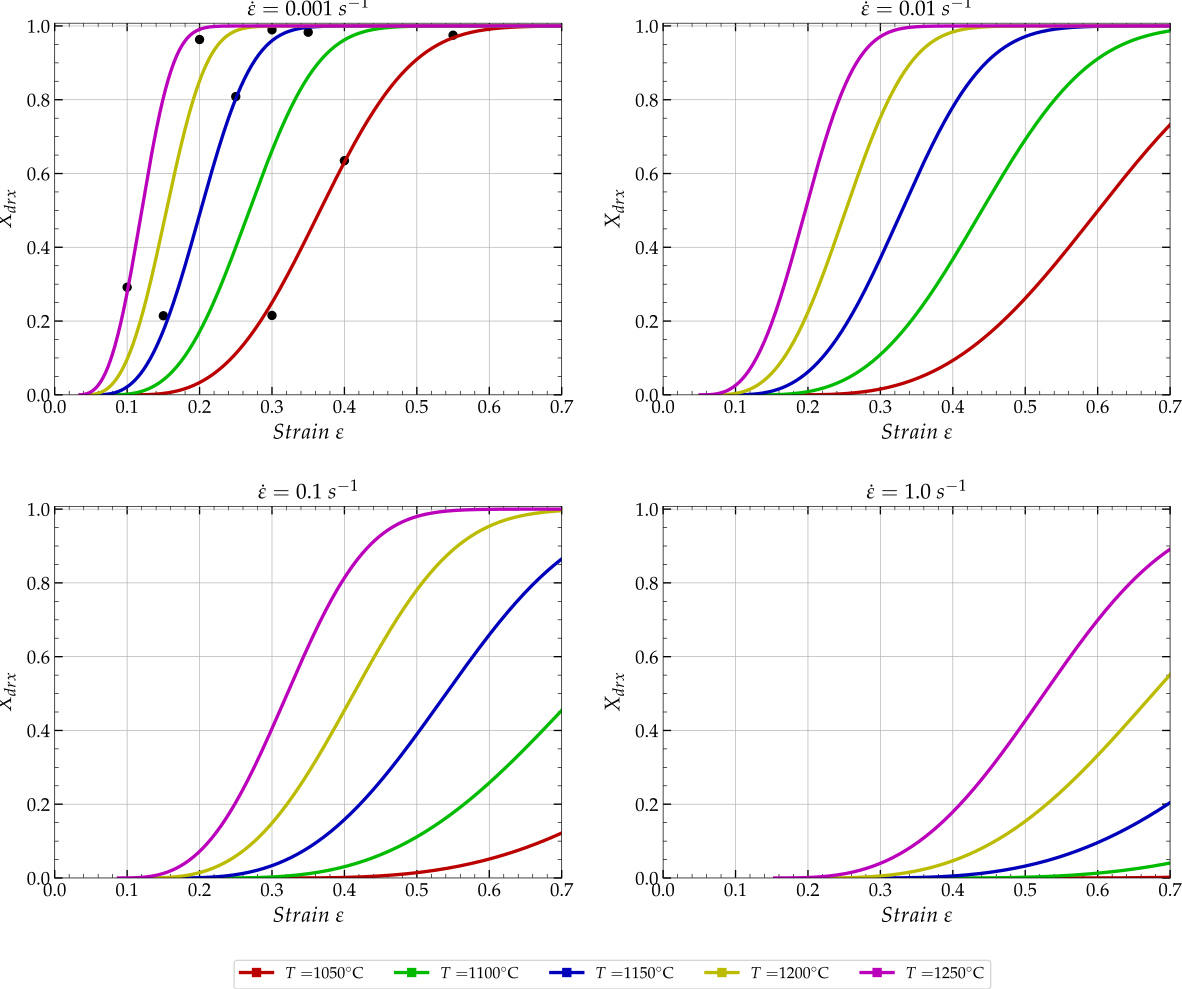
\includegraphics[width=0.99\columnwidth]{Figures/nDRX1}
	\caption{DRX experimental data (dots) and JMAK model based prediction (plain lines).}
	\label{fig:nDRX}
\end{figure}
Figure \ref{fig:eDRX} shows a micrograph of the sample for $\mdot\varepsilon=0.001~\ps$, $T=1050^\circ$C and $\varepsilon=0.55$. From this later, we determined the location of one of experimental point in Figure \ref{fig:nDRX} (the red one for $\varepsilon=0.55$). The same approach using different temperatures and strains is used to obtain the other experimental points reported in Figure \ref{fig:nDRX}.
\begin{figure}[H]
	\centering
	\includegraphics[width=0.5\columnwidth]{Figures/micrograph}
	\caption{Micrograph of the sample for $\mdot\varepsilon=0.001~\ps$, $T=1050^\circ$C and $\varepsilon=0.55$.}
	\label{fig:eDRX}
\end{figure}
The curves illustrate the changes in predicted volume fractions of DRX with plastic strain and it is evident that the proportion of DRX is strongly affected by strain, temperature, and strain rate values.
The DRX kinetics exhibit an S-shaped curve, with the DRX volume fraction gradually increasing with strain.
At a constant temperature and strain, the DRX volume fraction increases with decreasing strain rate.
Conversely, at a fixed strain rate and strain, the DRX volume fraction increases with rising temperature.
The difference between the predicted and experimental volume fractions of DRX is insignificant, confirming the suitability of the proposed approach for DRX prediction in the studied superalloy under various forming conditions.
The reduction of DRX with increasing strain rate can be attributed to the sensitivity of the volume fraction of dynamic recrystallization to forming temperature and strain rate.
Dynamic recrystallization is prone to occur at high forming temperatures and low strain rates due to increased grain boundary mobility.
However, because of the limited mobility of grain boundaries, the rate of dynamic recrystallization is slow at low forming temperatures and high strain rates.
The validation of the model used in the study, as evidenced by the correlation between experimental and predicted results, supports the subsequent use of these findings in the simulation section.

%----------------------------------------------------------------------------------
\section{Numerical simulation of the compression\label{sec:NumSim}}
%----------------------------------------------------------------------------------
In this section, we will focus on numerically validating the previously performed identification of dynamic recrystallization.
This requires establishing a constitutive law capable of accurately predicting the material's plastic deformation.
In our previous publication (Tize Mha \eal \cite{TizeMha-2023}), we conducted a comparison between analytical constitutive laws and a neural network-based approach.
The results revealed an artificial neural network model as the most appropriate option for this material.
As a result, this section has two main focuses: first, a summary of the ANN-based constitutive law identification, as previously presented; and second, the incorporation of this identified ANN model with the JMAK model to predict dynamic recrystallization behavior.

%----------------------------------------------------------------------------------
\subsection{Identification of the ANN constitutive law\label{subsec:ANNConstitutiveLaw}}
%----------------------------------------------------------------------------------

In general terms, flow stress $\sigma$ is a non-linear function of the strain $\varepsilon$, increasing with the strain rate $\mdot\varepsilon$, but decreasing with increasing temperature $T$.
This model can be described as an elastoplastic model that takes into consideration the influence of temperature and strain rate.
This type of behavior generally leads to Johnson--Cook \cite{Johnson-1983}, Zerilli--Armstrong \cite{Zerilli-1987}, Hansel--Spittel \cite{Hensel-1978}, PTM \cite{TizeMha-2023} or Arrhenius \cite{Sellars-1966} flow law type.
Depending on the nature of the stress-strain relationship, modeling with one or other of these models can take into account the actual behavior of the material at certain strain rates.

As stated in the research conducted by Tize Mha \eal \cite{TizeMha-2023}, the Johnson--Cook, Zerilli--Armstrong, or Hansel--Spittel models provide an estimate of material behavior at strain rates exceeding $1~\ps$, but they neglect the softening due to DRX that is evident on experimental curves for strain rates below $1~\ps$, as presented in Figure \ref{fig:RawData}.
Indeed, at the lowest strain rates, the flow stress $\sigma$ increases with strain $\varepsilon$ until reaching a value of roughly $\varepsilon=0.2$ to $0.3$.
Afterward, it decreases, maintaining a relatively constant value until the end of the compression test.
The Arrhenius model is the only one that can somewhat explain this softening at low strain rates.
As proposed by Pantalé \eal \cite{Pantale-2021} and Tize Mha \eal \cite{TizeMha-2023}, an effective alternative is to use a flow law defined by an artificial neural network trained directly on experimental data from compression tests.
Properly defining the hyper-parameters of this neural network, such as the number of hidden layers, number of neurons, and activation functions, enables us to obtain a flow law that accurately replicates the data acquired from compression tests.

According to the method proposed by Pantalé \eal \cite{Pantale-2021}, we have developed a two-hidden-layer artificial neural network based flow law in Tize Mha \eal \cite{TizeMha-2023}.
Figure \ref{fig:ANN-2HL} shows the general structure of this ANN.
The input layer of the ANN consists of three neurons that correspond to the model inputs, which are $\varepsilon$, $\mdot\varepsilon$, and $T$.
The output layer of the ANN contains one neuron representing $\sigma$, while there are two hidden layers.
All details regarding the artificial neural network, experimental data setup, and training method are detailed in the paper proposed by Pantalé \eal \cite{Pantale-2021}.

\begin{figure}[H]
\centering
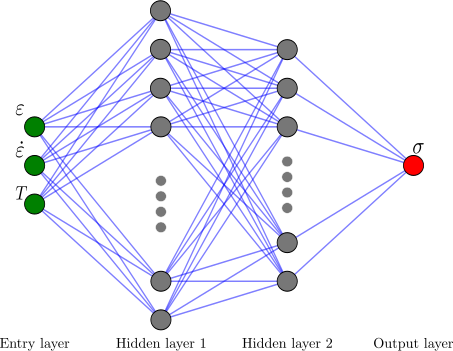
\includegraphics[width=0.55\columnwidth]{Figures/ANN-scheme-2HL}
\caption{Two hidden layers artificial neural network architecture with 3 inputs neurons (green) and 1 output neuron (red).}
\label{fig:ANN-2HL}
\end{figure}

We again used the Tensorflow library to develop the training program and employed the ADAM optimizer for the training phase.
The training database, as described in Section \ref{subsec:ExperimentalProcedure}, contains $21,030$ quadruples (we have $701\times30$ quadruples because $\varepsilon\in[0,0.7]$ with an increment of $0.001$, so we have $701$ values and 30 data curves) of values for strain ($\varepsilon$), strain rate ($\mdot\varepsilon$), temperature ($T$), and stress ($\sigma$).

We selected six different networks, named 3-$n$-$m$-1, where $n$ represents the number of neurons in the first hidden layer and $m$ indicates the number of neurons in the second hidden layer to demonstrate the significance of choosing the appropriate number of neurons in these two layers.

The training was conducted based on $5,000$ epochs of the experimental dataset.
It took 40 minutes to train the ANN model on a Dell XPS-13 7390 laptop running Ubuntu 22.04 LTS 64-bit operating system with 16 GB of RAM and an Intel 4-core i7-10510U processor until obtaining the converged parameters.

Figure \ref{fig:ANN-conv} shows the evolution of the training error, defined by the $\log_{10}$ of the internal $\RMSE$, during the training phase.
Table \ref{tab:Errors} summarizes the final values of this criterion, as well as the final values of the $\MARE$ and the $\RMSE$ for all six neural network configurations.
Based on these results, the 3-15-7-1 network was chosen for further investigation.
This network exhibited the most efficient convergence and achieved the lowest final error values of $\MARE=0.62\%$ and $\RMSE=0.38~\MPa$, while also maintaining a reasonable number of internal parameters ($N_{int}=180$).

\begin{figure}[H]
\centering
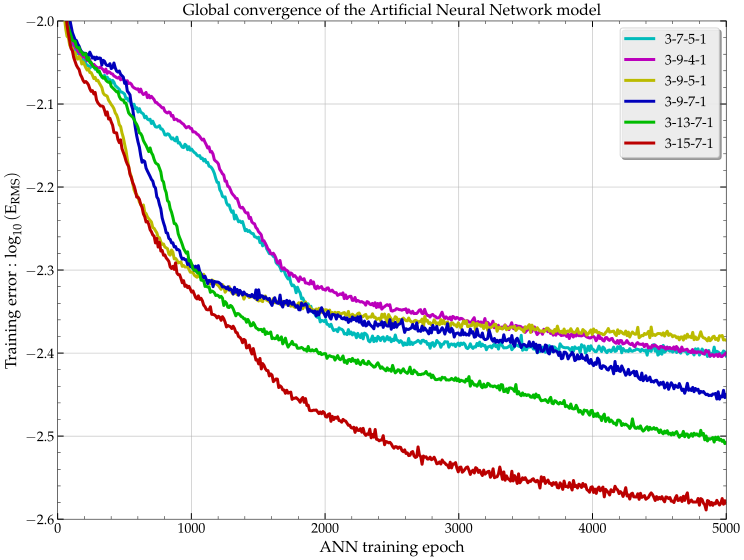
\includegraphics[width=0.7\columnwidth]{Figures/Conv-ANN-6}
\caption{Evolution of the convergence of the models during the training procedure for the 6 proposed network architectures.}
\label{fig:ANN-conv}
\end{figure}

\begin{table}[H]
\caption{Architecture and accuracy coefficients for all the proposed networks.}
\newcolumntype{C}{>{\centering\arraybackslash}X}
\newcolumntype{L}{>{\raggedright\arraybackslash}X}
\begin{tabularx}{\textwidth}{LCCCCCC}
\toprule
\textbf{Coefficients} & \textbf{3-7-5-1} & \textbf{3-9-4-1} & \textbf{3-9-5-1} & \textbf{3-9-7-1} & \textbf{3-13-7-1} & \textbf{3-15-7-1} \\
\toprule
$N_{int}$ & $74$ & $81$ & $92$ & $114$ & $158$ &$180$\\
\hline
$\log_{10}(\RMSE)$ & $-2.40$ & $-2.42$ & $-2.38$ & $-2.45$ & $-2.50$ & $-2.58$ \\
$\MARE(\%)$ & $1.13$ & $1.05$ & $1.08$ & $0.91$ & $0.75$ & $0.62$ \\
$\RMSE(\MPa)$ & $0.59$ & $0.57$ & $0.65$ & $0.55$ & $0.46$ & $0.38$ \\
\bottomrule
\end{tabularx}
\label{tab:Errors}
\end{table}

\begin{figure}[H]
\centering
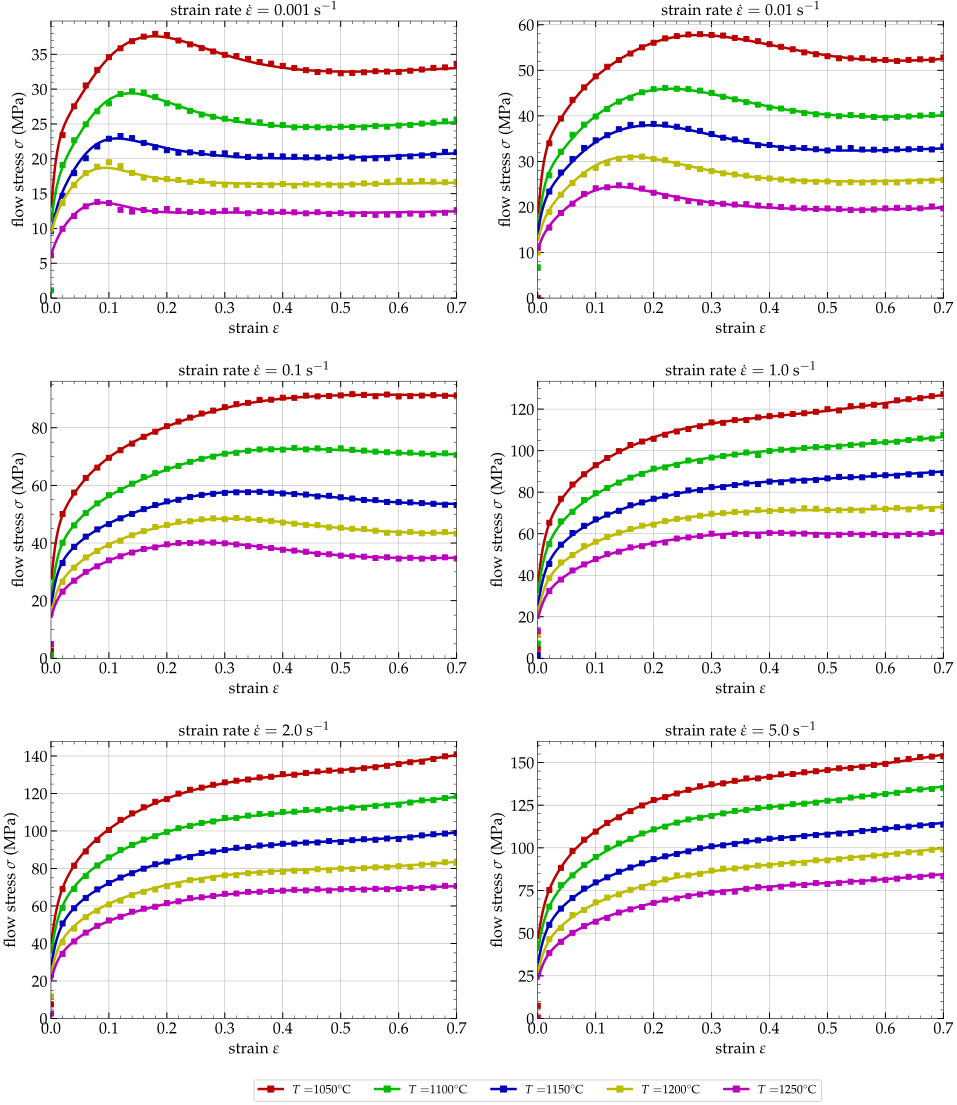
\includegraphics[width=0.9\columnwidth]{Figures/CompExpANN-3-15-7-1}
\caption{Comparison between the experimental (dots) and predicted (lines) flow stresses $\sigma$ by the 3-15-7-1 ANN model.}
\label{fig:ANN-3-15-7-1}
\end{figure}
This model will serve as the material flow equation for the numerical simulations discussed in Section \ref{subsec:DRXSimulation}.
Once the neural network is trained and a stable solution is obtained, it is re-implemented as a Fortran 77 VUHARD subroutine to calculate the material flow stress in the Abaqus FEM code. The details of the procedure and complete equations set required to calculate the flow stress $\sigma$ and the three derivatives of the flow stress with respect to $\varepsilon$, $\mdot{\varepsilon}$ and $T$ can be found in \cite{Pantale-2021}.

%----------------------------------------------------------------------------------
\subsection{Dynamic recrystallization simulation\label{subsec:DRXSimulation}}
%----------------------------------------------------------------------------------

To evaluate the effectiveness of the DRX model presented earlier, we propose a numerical simulation of a compression test in this section.
Our simulation concerns a medium-carbon P20 iron alloy, the same material used for the model's identification.
An axisymmetric Finite Element (FE) model of hot cylinder compression with a height of $h=15$~mm and a diameter of $\phi=10$~mm is used, as shown in Figure \ref{fig:Mesh}.
The assumed friction coefficient at the material/die interface is $\mu=0.2$ \cite{Zhang-2019,Sun-2020}.
The mesh is composed of $986$ ($17\times58$) CAX4R elements (4-node axisymmetric bi-linear quadrilateral elements with reduced integration and hourglass control).
Abaqus/Implicit is used to run the FE model simulation because of the long time needed to simulate a low strain rate compression.
A displacement of $60\%, ~45\%, ~30\%$ and $15\%$ of the total height is imposed on the upper part of the cylinder along the vertical axis of the specimen during compression.
The upper and the lower parts of the specimen can slip in the radial direction according to the friction coefficient and the contact conditions.
The axial displacement ($u_z$) of the upper part is imposed with a fixed velocity while the axial displacement of the lower part remains fixed during the simulation.
The simulation evaluated the impact of reducing the cylinder height with the effects of strain rate and temperature.
Conclusions were drawn based on this analysis.
The simulation considered three temperatures ($1050\degree$C, $1150\degree$C, and $1250\degree$C) and four strain rates ($0.001~\ps$, $0.01~\ps$, $0.1~\ps$, and $1.0~\ps$).
\begin{figure}[H]
\centering
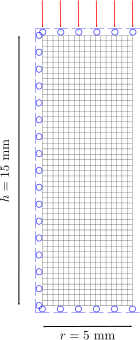
\includegraphics[height=0.7\columnwidth]{Figures/CyCompression2}
\caption{Numerical FE model for the simulation of the compression test.}
\label{fig:Mesh}
\end{figure}

%----------------------------------------------------------------------------------
\subsubsection{Temperature and strain rate effects \label{subsec:TempSReffect}}
%----------------------------------------------------------------------------------

Temperature and strain rate are critical factors that influence dynamic recrystallization in materials, particularly metals and alloys.
This process leads to the formation of new grains within the material.
Higher temperatures and lower strain rates typically result in increased nucleation rates and faster growth rates of new grains during dynamic recrystallization.
Conversely, lower temperatures and higher strain rates can lead to incomplete dynamic recrystallization.
At high temperatures, the increased mobility of both atoms and dislocations facilitates the formation of fresh grain boundaries and promotes the growth of new grains, resulting
in a more refined and isotropic grain structure.
In addition, higher temperatures can raise the proportion of recrystallized material, with the enhanced dislocation mobility contributing to new grain creation.
Consequently, this may result in a substantial change of the microstructure and the mechanical properties of the material.
Figure \ref{fig:TempEffect} and Figure \ref{fig:SREffect} display the simulated results of the DRX fraction of P20 steel under different deformation conditions.
Figure \ref{fig:TempEffect} shows that as the temperature increases, the extent of dynamic recrystallization widens.
The gradual increase in the dynamic recrystallization fraction in the center is noticeable, spreading outward.
This expansion is a result of higher thermal activation and increased atomic diffusion at higher temperatures, which makes the material more vulnerable to dynamic recrystallization.
The dynamic recrystallization degree ($X_{drx}$) unequivocally grows with the increase in temperature and reduction.
At $45\%$ and $60\%$ reduction, the $X_{drx}$ of P20 steel
attained $100\%$ in the center of the specimen at all the initial sample temperatures.
Indeed, the plastic deformation of a material is accompanied by the creation of dislocations.
These dislocations represent a "storage of elastic energy".
When the temperature is high enough, the dislocations become spontaneously mobile and cause a reorganization of the crystal structure in two stages: restoration and recrystallization.
The nature of the phases remains unchanged (those that are thermodynamically stable), and the atoms retain the same lattice.
However, the grain boundaries and the orientation of the crystallites undergo changes.

\begin{figure}[H]
\centering
\includegraphics[height=0.6\columnwidth]{Figures/Temp_DRX}
\caption{$X_{drx}$ values at a fixed strain rate of $\mdot{\varepsilon}=0.01~\ps$ for different reductions and initial temperatures $T_0$.}
\label{fig:TempEffect}
\end{figure}
\begin{figure}[H]
\centering
\includegraphics[height=0.6\columnwidth]{Figures/SR_DRX}
\caption{$X_{drx}$ values at a fixed $T_0=1150\celsius$ for different reductions and strain rates.}
\label{fig:SREffect}
\end{figure}

The temperature at which these phenomena occur depends on the rate of deformation.
The amount of elastic energy stored by a material increases with the degree of deformation, initiating restoration and recrystallization at a lower temperature.
As shown in Figure \ref{fig:SREffect}, escalating strain rates result in a decrease in the extent of recrystallization due to reduced dynamic recrystallization magnitude.
This result is due to the faster strain rate, which increases the critical strain and decreases the chance of internal dynamic recrystallization in the material.

%----------------------------------------------------------------------------------
\subsubsection{Experimental validation \label{subsec:ExpValid}}
%----------------------------------------------------------------------------------

In this section, we will compare experimental and simulation data by observing the dynamic recrystallization percentage of selected regions.
Figure \ref{fig:expNumDRX} shows the comparison between experimental data and simulation data for a test conducted at a temperature of $1150\celsius$ with a strain rate of $\mdot{\varepsilon}=0.1~\ps$.
Four zones were chosen to observe the percentage of recrystallization, ranging from $5\%$ to $100\%$.
The $5\%$ corresponds to the dead zone, representing the contact area between the sample and die experiencing friction effects.
In contrast, $100\%$ corresponds to the value observed at the center of the sample where deformation is the highest.
The temperature is elevated at the center of the sample, leading to a significant accumulation of energy.
Conversely, at the edges of the sample, a relatively complete recrystallization is observed.
This is because the temperature during deformation shifts from the center towards the upper and lower regions of the piece (due to the fact that the anvils are cooled), allowing recrystallization to occur.
Microscopic observations of each zone show large grains (Figure \ref{fig:expNumDRX} (d)) in the dead zone, while small grains (Figure \ref{fig:expNumDRX} (a)) are observed in the center of the sample, resulting from complete recrystallization.

\begin{figure}[H]
\centering
\includegraphics[width=0.98\columnwidth]{Figures/drxExpNum}
\caption{Experimental and numerical $X_{drx}$ values for $T_0=1150\celsius$ and strain rate $\mdot{\varepsilon}=0.1~\ps$}.
\label{fig:expNumDRX}
\end{figure}

%----------------------------------------------------------------------------------
\section{Conclusions\label{sec:Conclusions}}
%----------------------------------------------------------------------------------

In this study, we used the abilities of the ANN technique to deeply comprehend the dynamic recrystallization process and its adaptations in varying conditions.
Through the fusion of ANN modeling, fundamental material models, simulation software, and experimental confirmation, a comprehensive framework has been created that greatly enhances the materials science and engineering field.
Initially, we successfully used an ANN model to efficiently filter flow stress curves, which enabled us to predict critical conditions using the Poliak model.
This allows us to accurately anticipate the conditions at which the DRX process begins, providing a valuable tool for predicting material behavior under specific deformation scenarios.

We used the predicted critical conditions to input into the JMAK model, resulting in the successful prediction of the volume fraction of DRX and providing valuable insights into the kinetics and mechanisms controlling recrystallization.
This incorporation establishes a connection between theoretical models and practical phenomena, ultimately leading to a more deep comprehension of the complex processes occurring during deformation.
Taking our investigation further, we integrated the JMAK model into the widely-used ABAQUS software to simulate the evolution of DRX during hot compression tests.
This allowed us to capture the process's response to varying conditions without bias.
By comparing our simulation results with experimental data and using microstructure analysis, we have validated the accuracy of our simulations and confirmed the effectiveness of our predictive models.

It is noteworthy that although our research represents a significant milestone, it also presents opportunities for future exploration.
Further enhancing the accuracy and applicability of our predictions can be achieved by fine-tuning our model, expanding our dataset, and refining the integration process.
Moreover, the successful connection of theory, simulation, and experimentation offers a sturdy structure for addressing challenging material behavior issues in industries ranging from manufacturing to aerospace or other applications.

%%%%%%%%%%%%%%%%%%%%%%%%%%%%%%%%%%%%%%%%%%
%\section{Patents}

%%%%%%%%%%%%%%%%%%%%%%%%%%%%%%%%%%%%%%%%%%
\vspace{6pt}

%%%%%%%%%%%%%%%%%%%%%%%%%%%%%%%%%%%%%%%%%%
%% optional
%\supplementary{The following supporting information can be downloaded at: \linksupplementary{s1}, Figure S1: title; Table S1: title; Video S1: title.}

% Only for the journal Methods and Protocols:
% If you wish to submit a video article, please do so with any other supplementary material.
% \supplementary{The following supporting information can be downloaded at: \linksupplementary{s1}, Figure S1: title; Table S1: title; Video S1: title. A supporting video article is available at doi: link.}

%%%%%%%%%%%%%%%%%%%%%%%%%%%%%%%%%%%%%%%%%%
\authorcontributions{
Conceptualization, P.T.M. and O.P.;
methodology, O.P.;
software, P.T.M. and O.P.;
validation, O.P.;
formal analysis, O.P. and P.D.;
investigation, P.D.;
resources, P.D. and M.J.;
data curation, P.T.M. and P.D.;
writing---original draft preparation, O.P. and P.T.M.;
writing---review and editing, O.P.;
visualization, O.P.;
supervision, M.J., A.T. and O.P.;
project administration, M.J.;
funding acquisition, M.J.
All authors have read and agreed to the published version of the manuscript.}

\funding{This work was supported by the Natural Sciences and Engineering Research Council of Canada (NSERC) in the framework of a Collaborative Research and Development project (CRD) (Grant Number 5364418).}

%\institutionalreview{In this section, you should add the Institutional Review Board Statement and approval number, if relevant to your study. You might choose to exclude this statement if the study did not require ethical approval. Please note that the Editorial Office might ask you for further information. Please add “The study was conducted in accordance with the Declaration of Helsinki, and approved by the Institutional Review Board (or Ethics Committee) of NAME OF INSTITUTE (protocol code XXX and date of approval).” for studies involving humans. OR “The animal study protocol was approved by the Institutional Review Board (or Ethics Committee) of NAME OF INSTITUTE (protocol code XXX and date of approval).” for studies involving animals. OR “Ethical review and approval were waived for this study due to REASON (please provide a detailed justification).” OR “Not applicable” for studies not involving humans or animals.}

%\informedconsent{Any research article describing a study involving humans should contain this statement. Please add ``Informed consent was obtained from all subjects involved in the study.'' OR ``Patient consent was waived due to REASON (please provide a detailed justification).'' OR ``Not applicable'' for studies not involving humans. You might also choose to exclude this statement if the study did not involve humans.
%
%Written informed consent for publication must be obtained from participating patients who can be identified (including by the patients themselves). Please state ``Written informed consent has been obtained from the patient(s) to publish this paper'' if applicable.}

\dataavailability{The raw/processed data required to reproduce these findings cannot be shared at this time due to privacy and ethical concerns.}

\acknowledgments{The authors acknowledge Jean-Benoit Morin, Director of Metallurgy and Quality from Finkl Steel-Sorel, Abdelhalim Loucif from the R\&D department of Finkl Steel-Sorel, Ecole de Technologie Superieure, and Ecole Nationale d'Ingenieurs de Tarbes, France, for providing technical data, materials, and testing facilities.}%MDPI: We removed titles here: OK

\conflictsofinterest{The authors declare no conflict of interest.}

%%%%%%%%%%%%%%%%%%%%%%%%%%%%%%%%%%%%%%%%%%
%% Optional
%\sampleavailability{Samples of the compounds ... are available from the authors.}

%% Only for journal Encyclopedia
%\entrylink{The Link to this entry published on the encyclopedia platform.}

\abbreviations{Abbreviations}{
The following abbreviations are used in this manuscript:\\

\noindent
\begin{tabular}{@{}ll}
ANN & Artificial neural network \\
AR  & Arrhenius \\
CPU & Central processing unit \\
DRC & Dynamic recovery\\
DRX & Dynamic recrystallization \\
$X_{drx}^{e,p}$ & DRX's Volume fraction : $e, p$ for experimental and prediction respectively \\
FE  & Finite Element \\
HS  & Hansel--Spittel \\
JC  & Johnson--Cook \\
MZA & Modified Zerilli--Armstrong \\
SRX & Static recrystallization \\
WH  & Work hardening \\
ZA  & Zerilli--Armstrong
\end{tabular}
}

%%%%%%%%%%%%%%%%%%%%%%%%%%%%%%%%%%%%%%%%%%
%% Optional
\appendixtitles{no} % Leave argument "no" if all appendix headings stay EMPTY (then no dot is printed after "Appendix A"). If the appendix sections contain a heading then change the argument to "yes".
\appendixstart
\appendix
\section[\appendixname~\thesection]{}\label{sec:Appendix}

%%%%%%%%%%%%%%%%%%%%%%%%%%%%%%%%%%%%%%%%%%
\begin{adjustwidth}{-\extralength}{0cm}
%\printendnotes[custom] % Un-comment to print a list of endnotes

\reftitle{References}

% Please provide either the correct journal abbreviation (e.g. according to the “List of Title Word Abbreviations” http://www.issn.org/services/online-services/access-to-the-ltwa/) or the full name of the journal.
% Citations and References in Supplementary files are permitted provided that they also appear in the reference list here.

%=====================================
% References, variant A: external bibliography
%=====================================
\bibliography{bibliography}

% If authors have biography, please use the format below
%\section*{Short Biography of Authors}
%\bio
%{\raisebox{-0.35cm}{\includegraphics[width=3.5cm,height=5.3cm,clip,keepaspectratio]{Definitions/author1.pdf}}}
%{\textbf{Firstname Lastname} Biography of first author}
%
%\bio
%{\raisebox{-0.35cm}{\includegraphics[width=3.5cm,height=5.3cm,clip,keepaspectratio]{Definitions/author2.jpg}}}
%{\textbf{Firstname Lastname} Biography of second author}

% For the MDPI journals use author-date citation, please follow the formatting guidelines on http://www.mdpi.com/authors/references
% To cite two works by the same author: \citeauthor{ref-journal-1a} (\citeyear{ref-journal-1a}, \citeyear{ref-journal-1b}). This produces: Whittaker (1967, 1975)
% To cite two works by the same author with specific pages: \citeauthor{ref-journal-3a} (\citeyear{ref-journal-3a}, p. 328; \citeyear{ref-journal-3b}, p.475). This produces: Wong (1999, p. 328; 2000, p. 475)

%%%%%%%%%%%%%%%%%%%%%%%%%%%%%%%%%%%%%%%%%%
%% for journal Sci
%\reviewreports{\\
%Reviewer 1 comments and authors’ response\\
%Reviewer 2 comments and authors’ response\\
%Reviewer 3 comments and authors’ response
%}
%%%%%%%%%%%%%%%%%%%%%%%%%%%%%%%%%%%%%%%%%%
\PublishersNote{}
\end{adjustwidth}
\end{document}

